\chapter{Introduction} 
This essay will be focusing on stencil computation and its development over the recent years due to the complex nature of modern computer architectures involving chip multicore processors (CMP) and heterogeneous system architectures. I will give a thorough description of stencil computation, CMP-systems as well as parallelization of such problems, and methods and optimizations on structured meshes

Stencil computations are operations performed by many numerical methods in the context of scientific  applications. A \textit{stencil} is a geometric pattern of a nodal group centered around some point using information from its neighbor elements, as shown in figure \ref{I_Five_point_stencil_illustration.png}. A stencil operation can be done over a mesh using series of time sweeps to update its value using neighboring values at which the stencil is centered.
\begin{figure}[h]
 \centering 
     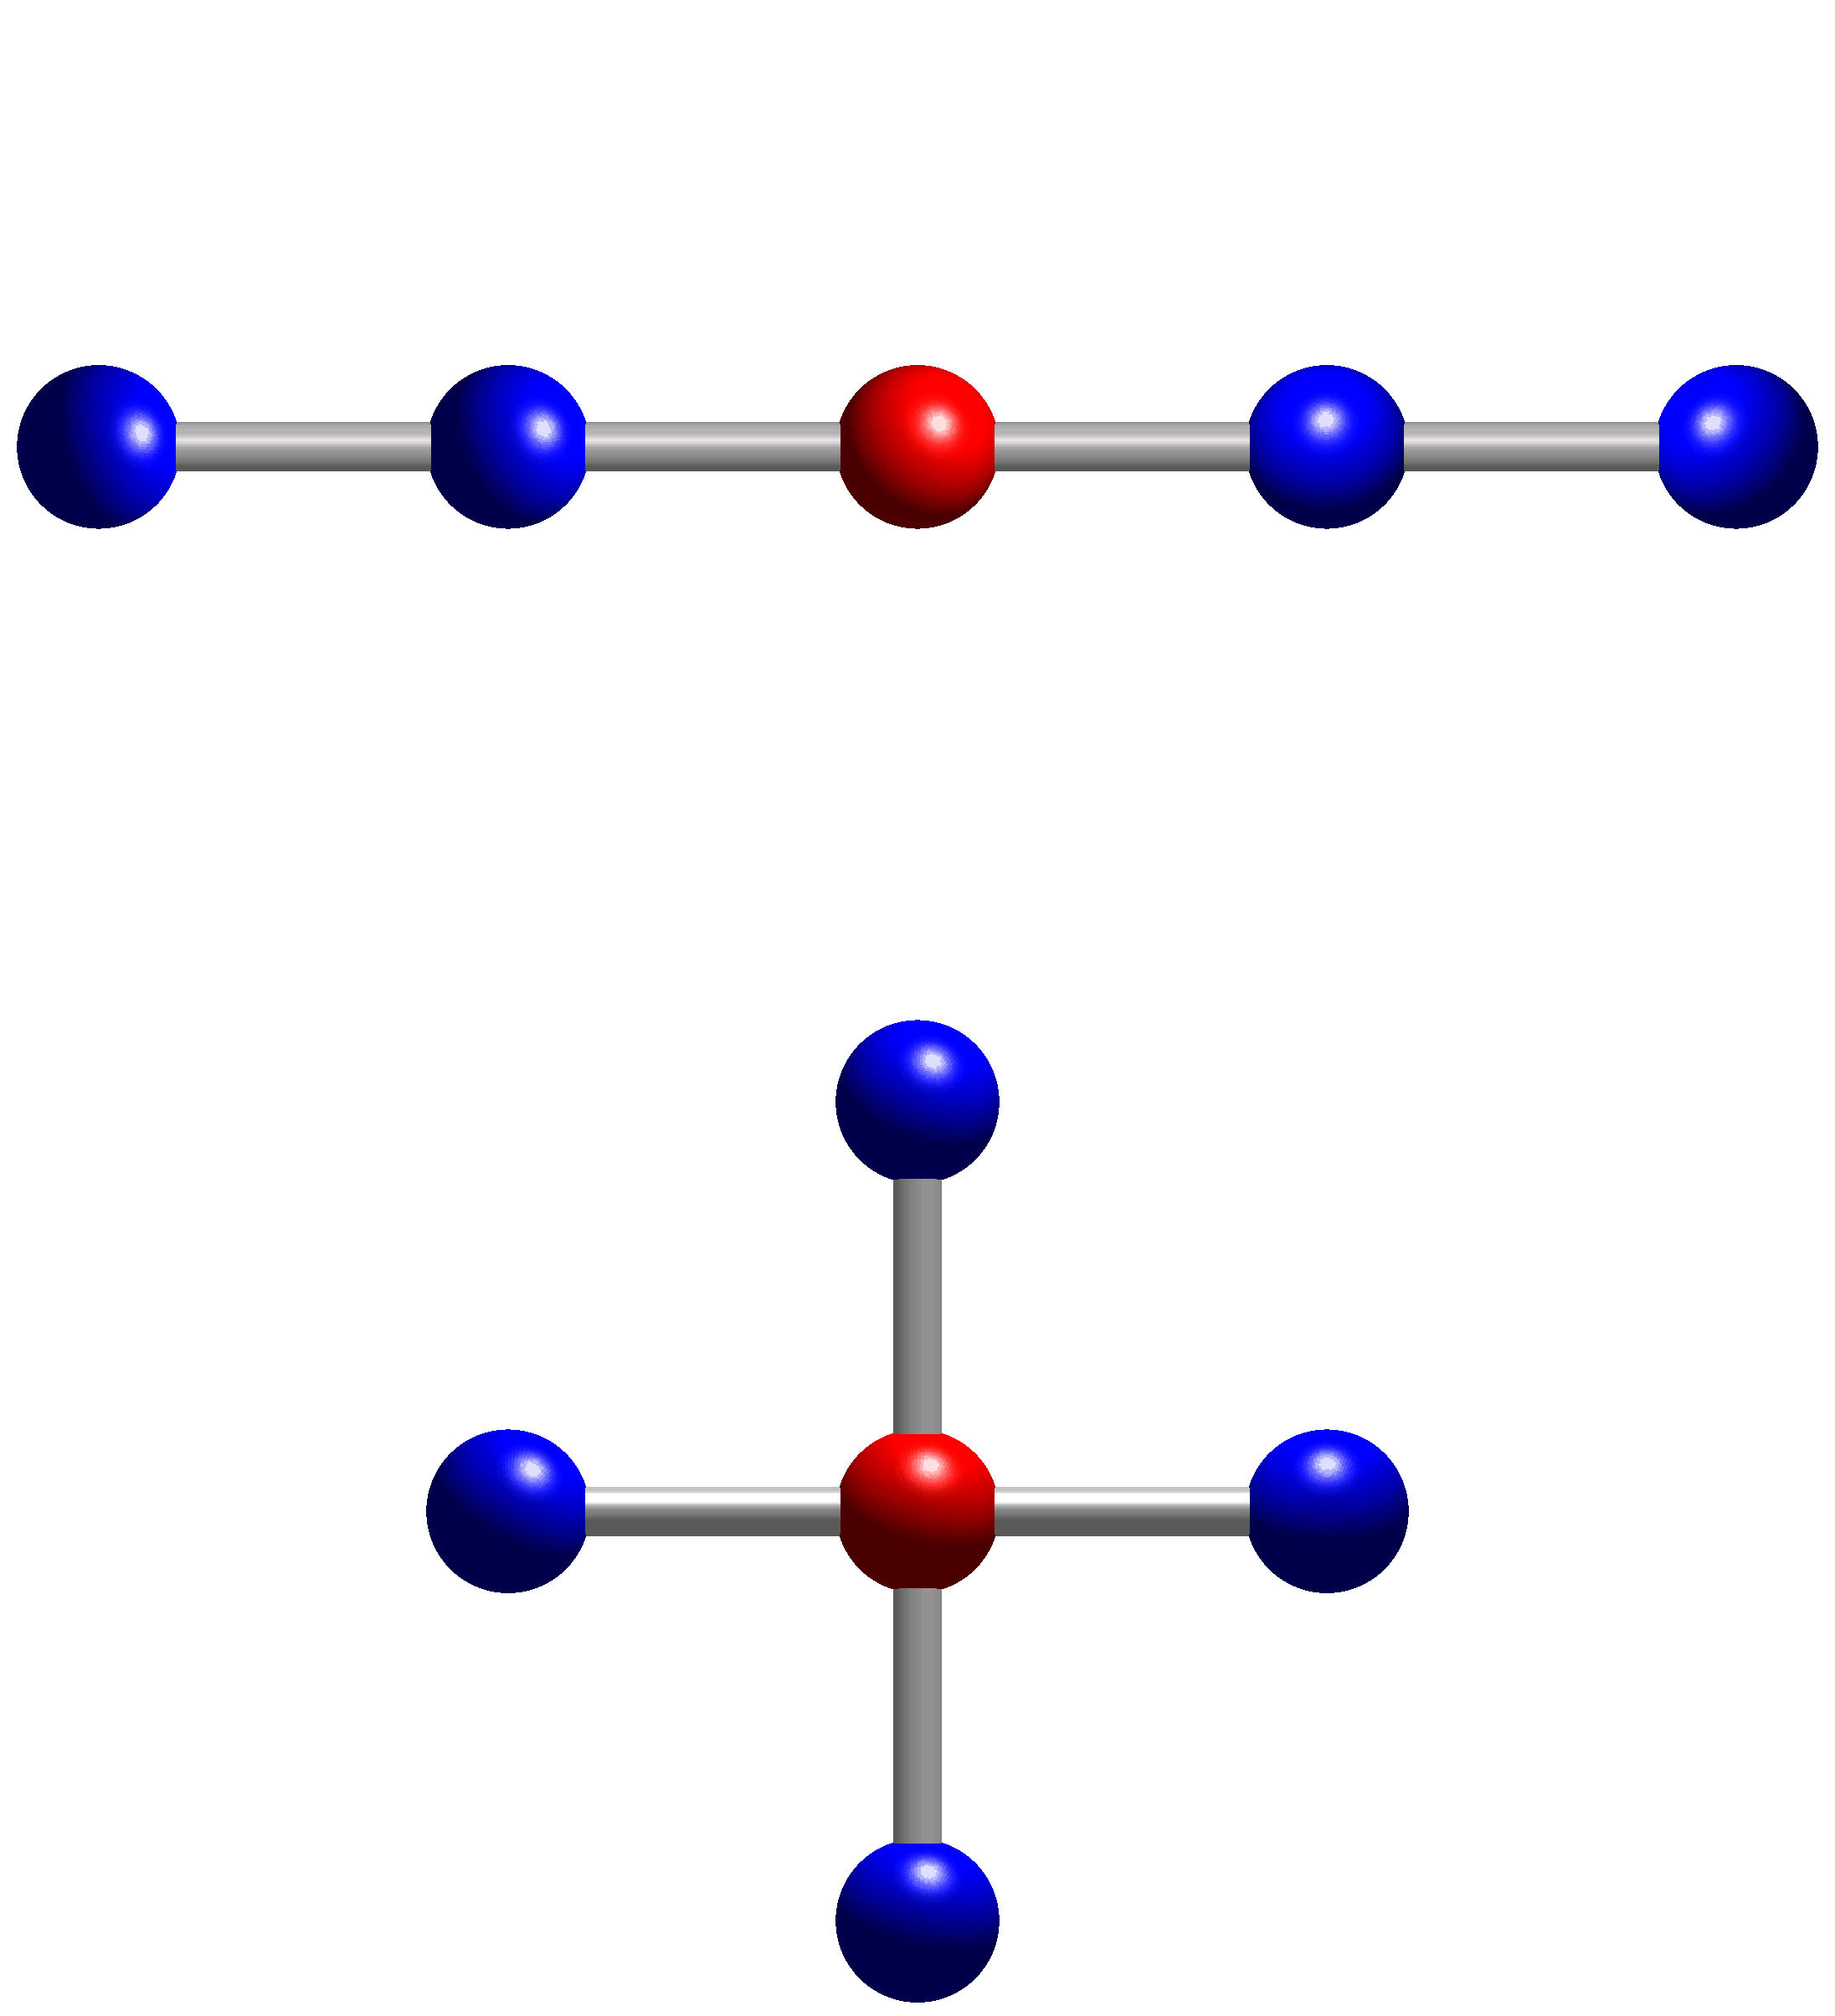
\includegraphics[height=0.5\textwidth]{bilder/I_Five_point_stencil_illustration}
     \caption{1 and 2 dimensional overview of two different 5-point stencils. Illustration taken form \cite{pic1}
     \label{I_Five_point_stencil_illustration.png}}
\end{figure}
A widely used numerical method such as the Finite Difference Method (FDM) are defined to operate over a mesh. I will dive deeper into iterative methods, which are methods used in numerical analysis, in section \ref{subsec:stencil_iteration_types}. 

A mesh is a collection of vertices, edges and faces \footnote{A vertex is a point in the coordinate system, an edge is the connection between two vertices, and a face is a closed set of edges, forming a surface} \cite{article15} that form a polygon mesh. A mesh can be classified as either \textit{structured} or \textit{unstructured}. A structured mesh is identified by a regular connectivity in the mesh pattern. A mesh pattern refers to the geometric alignment of the individual cells in the mesh. Possible element choices for a structured mesh are quadrilateral in 2D or hexahedra in 3D. Structured meshes are easier to evaluate, allow for easy parallelization, and generally require no spatial data structure to manage \cite{article2}. Unstructured meshes are identified by irregular connectivity in the mesh pattern, and can usually be seen as triangles in 2D and tetrahedra in 3D. Unstructured meshes offer the advantage of easier discretization of complex geometries. However they are harder to evaluate, often requiring additional overhead in the form of some spatial data structure, and are generally more difficult to parallelize \cite{article2}, due to its irregular connectivity in the mesh pattern. 
\begin{figure}[!h]
  \begin{center}
    \label{I_structured_mesh.png}
    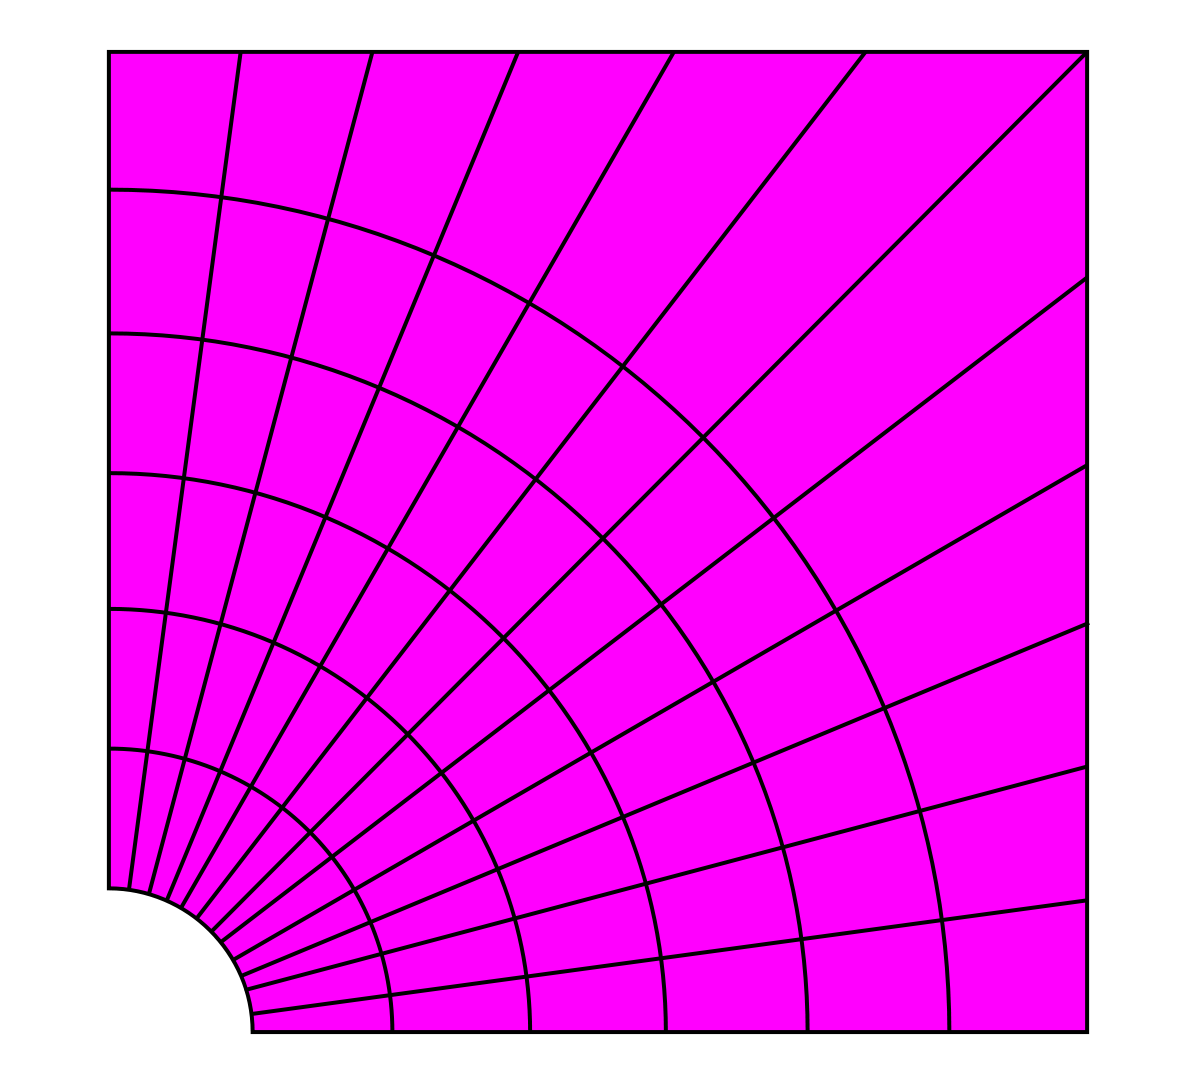
\includegraphics[width=0.45\textwidth]{bilder/I_structured_mesh}
    \label{I_unstructured_mesh.png}
    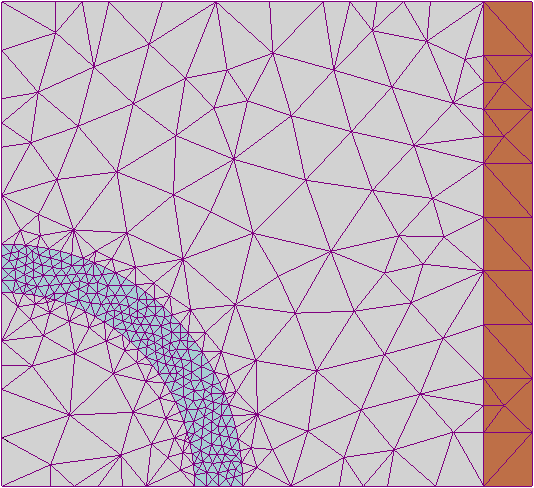
\includegraphics[width=0.45\textwidth]{bilder/I_unstructured_mesh}
  \end{center}
  \caption{Illustration of a structured and unstructured mesh, respectively. Taken from \cite{pic2} and \cite{pic3}}
  \label{I_mesh_types}
\end{figure}

Computations over structured meshes incur regular memory accesses that are easier to achieve, among other things, good cache performance. In comparison, unstructured meshes will include irregular and indirect memory accesses, which are challenging with respect to cache utilization.
A contiguous underlying data storage means that data elements are laid out end-to-end in the memory, with no discontinuities and padding between them, resulting in good memory patterns and high memory efficiency. A few techniques for assuring contiguous memory data storage involves dynamic memory allocation, and loop interchange. Optimization techniques will be discussed in greater detail in section \ref{sec:optimization}. 

%% Computations over structured meshes incur regular memory accesses that are easier to achieve, among other things, good cache performance 

%%as a result, structured meshes generally leads to contiguous memory access, good memory layout patterns, and high cache efficiency \cite{article2}.

%%Computations over structured meshes incur regular memory accesses that are easier to achieve, among other things, good cache performance. In comparison, unstructured meshes will include irregular and indirect memory accesses, which are challenging with respect to cache utilisation.

%%due to the simplicity in the mesh pattern compared to unstructured meshes, structured meshes generally leads to contiguous memory, which results in good memory layout patterns, and high cache efficiency

%%Structured meshes generally leads to contiguous memory, good memory layout patterns, and high cache efficiency \cite{article2}.
%%This essay will be focusing on methods and optimizations over structured meshes

%%Stencil computations performed over unstructured meshes are generally much harder than those performed over structured meshes, and they often exhibit non-contiguous memory access patterns and lower cache efficiency \cite{article2}, since it calls for explicit storage of neighborhood relationships \cite{article3}.

%%In this essay I will be focusing on methods and optimizations over unstructured meshes as they have 
%%\textcolor{red}{videre tanker etc.)}

%%optimization techniques will be discussed in greater detail in section \ref{sec:optimization}
%% \textcolor{red}{(called a localized region fjerne?)}

